\section{Construção de um exemplo}

Usando dados de um ensaio clínico, construiu-se um modelo de aprendizagem de máquina para predizer o nível de resposta à intervenção sendo testada.
Durante o processo de construção, optou-se pela utilização de técnicas simples, colocando a didática acima do desempenho preditivo.

\subsection{O estudo original}

O estudo original buscava avaliar o impacto de intervenções de psicologia positiva conduzidas via internet sobre a percepção de felicidade e
sintomas depressivos \cite{Woodworth2017}, uma tentativa de replicar os resultados obtidos em um trabalho anterior conduzido por Seligman e
colaboradores \cite{Seligman2005}.

\subsubsection{Participantes}

Os participantes foram recrutados por meio de anúncios em veículos de comunicação australianos: páginas web, jornais e uma estação de rádio
local. Um total de 295 participantes completou a fase inicial de pré-teste. O grupo era composto majoritariamente por mulheres ($85,06\%$),
com idades entre 18 e 83 anos ($M=43,76; SD=12,43$); a maior parte dos participantes possuia nível de educação superior ($74,88\%$) e classificou
a própria renda como média ou acima da média ($76\%$) \cite{Woodworth2017, Collins2023}.

\subsubsection{Intervenções}

Os participantes foram distribuídos aleatoriamente em quatro grupos, três grupos experimentais e um grupo de controle; cada um dos três grupos
experimentais recebeu uma intervenção distinta. O primeiro grupo experimental recebeu a intervenção de \emph{visita da gratidão}: os participantes
foram instruídos escrever e entregar uma carta de agradecimento para alguém que lhes tivesse sido gentil no passado. O segundo grupo experimental
recebeu a intervenção de \emph{três coisas boas}: os participantes deveriam anotar três coisas boas que haviam acontecido durante seu dia, justificando
suas escolhas de eventos. O último grupo experimental recebeu a intervenção de \emph{pontos fortes}: os participantes receberam uma intevenção
psicoeducativa sobre forças de caráter e foram aconselhados a buscar maneiras criativas para utilizar suas próprias forças de caráter no cotidiano.
Todas as intervenções tiveram duração de uma semana \cite{Woodworth2017}.

\subsubsection{Controle}

O grupo de controle foi exposto à atividade placebo de \emph{memórias de infância}: os participantes receberam a instrução de reservar um momento ao
final do dia para escrever sobre suas memórias de infância durante uma semana \cite{Woodworth2017}.

\subsubsection{Desfechos}

O estudo avaliou percepção de felicidade por meio do AHI (Authentic Happiness Inventory), um instrumento de autorrelato composto por 24 items. Os itens
são pontuados em uma escala de que vai de 1 a 5 e a pontuação total é calculada pela soma das pontuações obtidas para cada item. Resultados maiores representam
maiores níveis de felicidade \cite{Park2010}.

Sintomas depressivos foram mensurados com a escala CES-D (Center for epidemiologic studies depression scale), um instrumento de autorrelato composto por 20
itens que avaliam a frequência de sintomas em uma escala Likert de 4 pontos. A CES-D é divida em quatro subescalas: afeto deprimido, afeto positivo, queixas
somáticas e problemas interpessoais. A pontuação em uma subescala é calculada pela soma das pontuações obtidas para cada item associado à subescala. A pontuação
total é calculada pela soma das pontuações obtidas para cada subescala. Resultados maiores representam maior severidade dos sintomas depressivos \cite{Radloff1977}.

O estudo também coletou informação sobre sexo, idade, nível de escolaridade e renda das participantes. As medidas foram obtidas nas ocasiões de pré-teste, pós-teste
e 4 ocasiões de follow-up: uma semana após o pós-teste, um mês após o pós-teste, três meses após o pós-teste e seis meses após o pós-teste \cite{Woodworth2017}.

\subsection{Árvores de decisão}

Árvores de decisão representam uma classe de modelos de aprendizagem de máquina que pode ser usada para tarefas de classificação e regressão, ou seja, são
capazes de fazer predições para valores de variáveis categóricas e numéricas. Elas utilizam uma série de regras de decisão para predizer o desfecho de interesse;
essas regras consistem em verificações feitas sobre os valores de variáveis presentes no conjunto de dados usados no treinamento do modelo \cite{Theobald2021, Bi2019}.

\begin{figure}[h!]
    \centering
    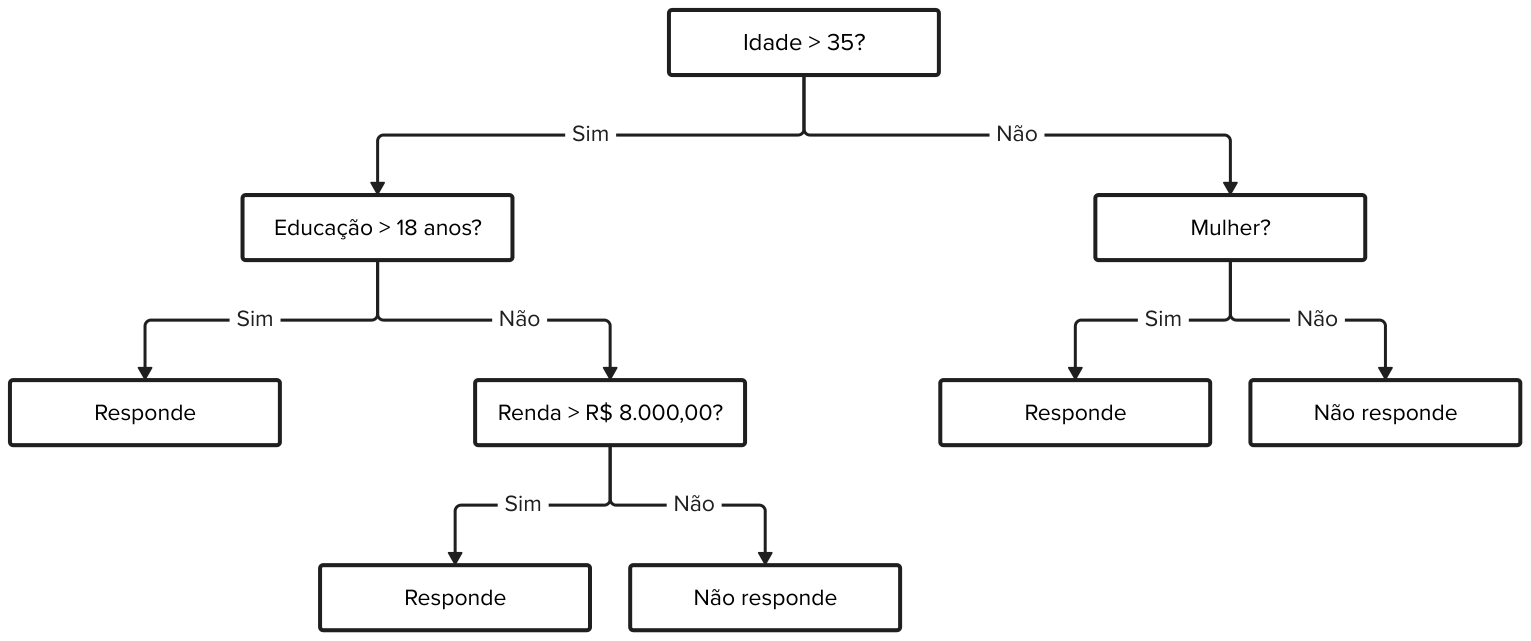
\includegraphics[width=\textwidth]{./03-exemplo/imagens/arvore-exemplo.png}
    \caption{Um exemplo de árvore de decisão construída manualmente.}
    \label{fig:arvore-exemplo}
\end{figure}

Na figura \ref{fig:arvore-exemplo}, tem-se uma árvore de decisão construída manualmente que realiza a tarefa de predição da resposta a uma intervenção psicoterápica hipotética.
Com acesso às informações necessárias, é possível navegar pela estrutura da árvore e predizer o desfecho que a inteverção teria para uma nova paciente. Para isso, aplicam-se
as regras de decisão sucessivamente a partir do nó inicial, chamado raiz, até alcançar um nó terminal, chamado folha, que contém a informação de desfecho.  Por exemplo,
uma paciente de 38 anos, que estudou durante 15 anos de sua vida e tem uma renda mensal de R\$ $10.000,00$ teria uma previsão de desfecho com resposta positiva à intervenção.

Algoritmos de aprendizagem de máquina para construção de árvores de decisão operam por meio de um processo iterativo: o processamento do conjunto de dados de treinamento
acontece em ciclos que se repetem um determinado número de vezes. Partindo do conjunto de dados de treinamento completo, geram-se as regras de decisão possíveis e seleciona-se
aquela que produz partições mais homogêneas dos dados em relação ao desfecho de interesse. As particões geradas servem como base para o próximo ciclo de processamento. O processo
segue até que se alcance um critério de parada pré-estabelecido, como o tamanho da árvore ou um número mínimo de observações em nós terminais \cite{Bi2019}.

O uso de árvores de decisão apresenta uma série de benefícios. Árvores de decisão exigem um volume de dados menor para realização do treinamento quando comparadas a outras classes
de modelos como as redes neurais artificiais \cite{Theobald2021}. Elas são capazes de modelar relações não lineares entre as variáveis do conjunto de dados, desempenhando melhor
que modelos de regressão linear em contextos onde esse tipo de interação existe \cite{Bi2019}. Além disso, árvore de decisão são facilmente interpretáveis; elas possuem uma representação
gráfica que pode ser compreendida de maneira intutiva, facilitando sua inspeção e a obtenção de insights sobre o processo de tomada de decisão empregado pelo modelo \cite{Bi2019}.
As limitações de modelos de árvore de decisão incluem sua sensibilidade a pequenas perturbações no conjunto de dados, como outliers, e uma inclinação ao sobreajuste: uma adaptação
excessiva às nuances do conjunto de dados de treinamento que prejudica a capacidade de generalização das predições feitas pelo modelo \cite{Bi2019}.

\subsection{Plano de análise de dados}

Construiu-se um modelo de aprendizagem de máquina do tipo árvore de decisão para predizer melhora nos níveis de sintomas depressivos a nível individual após a intervenção.
Foram utilizados a linguagem de programação Python na versão 3.12 \cite{Python} e o pacote para processamento estatístico e de aprendizagem de máquina scikit-learn na versão
1.5 \cite{ScikitLearn}.

O conjunto de dados do estudo original, que incluia observações sobre diversas ocasiões de follow-up, foi filtrado para obter somente as observações de pré-teste e pós-teste; os dados de
pré-teste e pós-teste de cada participante foram combinados para compor uma única observação. A partir dos dados de pré-teste, foram mantidas as variáveis sociodemográficas (sexo, idade,
nível de educação e renda), pontuação em cada item do instrumento AHI, pontuação total no instrumento AHI, pontuação em cada item do instrumento CES-D e pontuação total no instrumento CES-D.
Para os dados de pós-teste, foi mantida a variável de pontuação total no instrumento CES-D. Observações relacionadas a participantes do grupo de controle foram descartadas. Após os tratamentos
iniciais o conjunto de dados disponíveis para a construção do modelo tinha 102 observações.

Adicionou-se uma variável catagórica para indicar melhora nos níveis de sintomas depressivos. A variável teve seu valor preenchido a partir da variação na pontuação total no instrumento CES-D:
participantes que apresentaram um aumento de cinco pontos no pós-teste em relação ao pré-teste receberam a classificação de respondentes ao tratamento; os demais participantes receberam a
classificação de não respondentes.

Separou-se aleatoriamente $20\%$ das observações disponíveis para compor o conjunto de dados de teste; os $80\%$ restantes foram utilizados para o treinamento do modelo de árvore de decisão.
O critério estabelecido para a seleção de regras de decisão foi o de entropia de Shannon \cite{ScikitLearn} e a profundidade máxima permitida para a árvore resultante foi de cinco níveis.

Utilizou-se o modelo na predição de desfechos para o conjunto de dados de testes, mantido em separado até então, e seu desempenho foi avaliado por meio das métricas de acurácia, precisão e
recall. Acurácia representa o percentual de predições corretas realizadas pelo modelo de modo geral. Precisão refere-se à razão entre classificações positivas corretas e o total de classificações
positivas feitas pelo modelo. Recall refere-se à razão entre as classificações positivas corretas e o total de observações positivas no conjunto de dados de teste.

\subsection{Resultados e discussão}

O modelo de árvore de decisão gerado é apresentado na figura \ref{fig:arvore}. O modelo conta com 17 nós organizados em uma estrutura com cinco níveis de profundidade sendo um nó raiz, sete
nós intermediários e nove nós folha. As regras de decisão selecionadas verificam os valores de oito variáveis distintas: a pontuação total no CES-D, a pontuação nos itens 13 e 19 do CES-D,
a pontuação nos itens 7, 15, 20 e 22 do AHI e a renda da participante. O item 13 da CES-D diz respeito a falar menos que o usual; o item 19 do instrumento refere-se ao sentimento de não ser
apreciado por outras pessoas. Os itens 7, 15, 20 e 22 da AHI referem-se respectivamente a sentimentos de tédio, satisfação com o trabalho, bom uso do tempo e experiências de prazer e dor.
Além da regra de decisão selecionada, o diagrama apresenta, para cada nó, informações sobre as partições geradas durante o processo de treinamento: o número de observações que alcançaram o
nó (samples), o nível de entropia de Shannon para as observações (entropy), a distribuição das observações entre as classes não respondente e respondente respectivamente (value) e a classe
predominante nas observações (class). A coloração dos nós no diagrama indica a classe predita pelo modelo, com a cor laranja representando participantes não respondentes e a cor azul representando
participantes respondentes.

\begin{figure}[h]
    \centering
    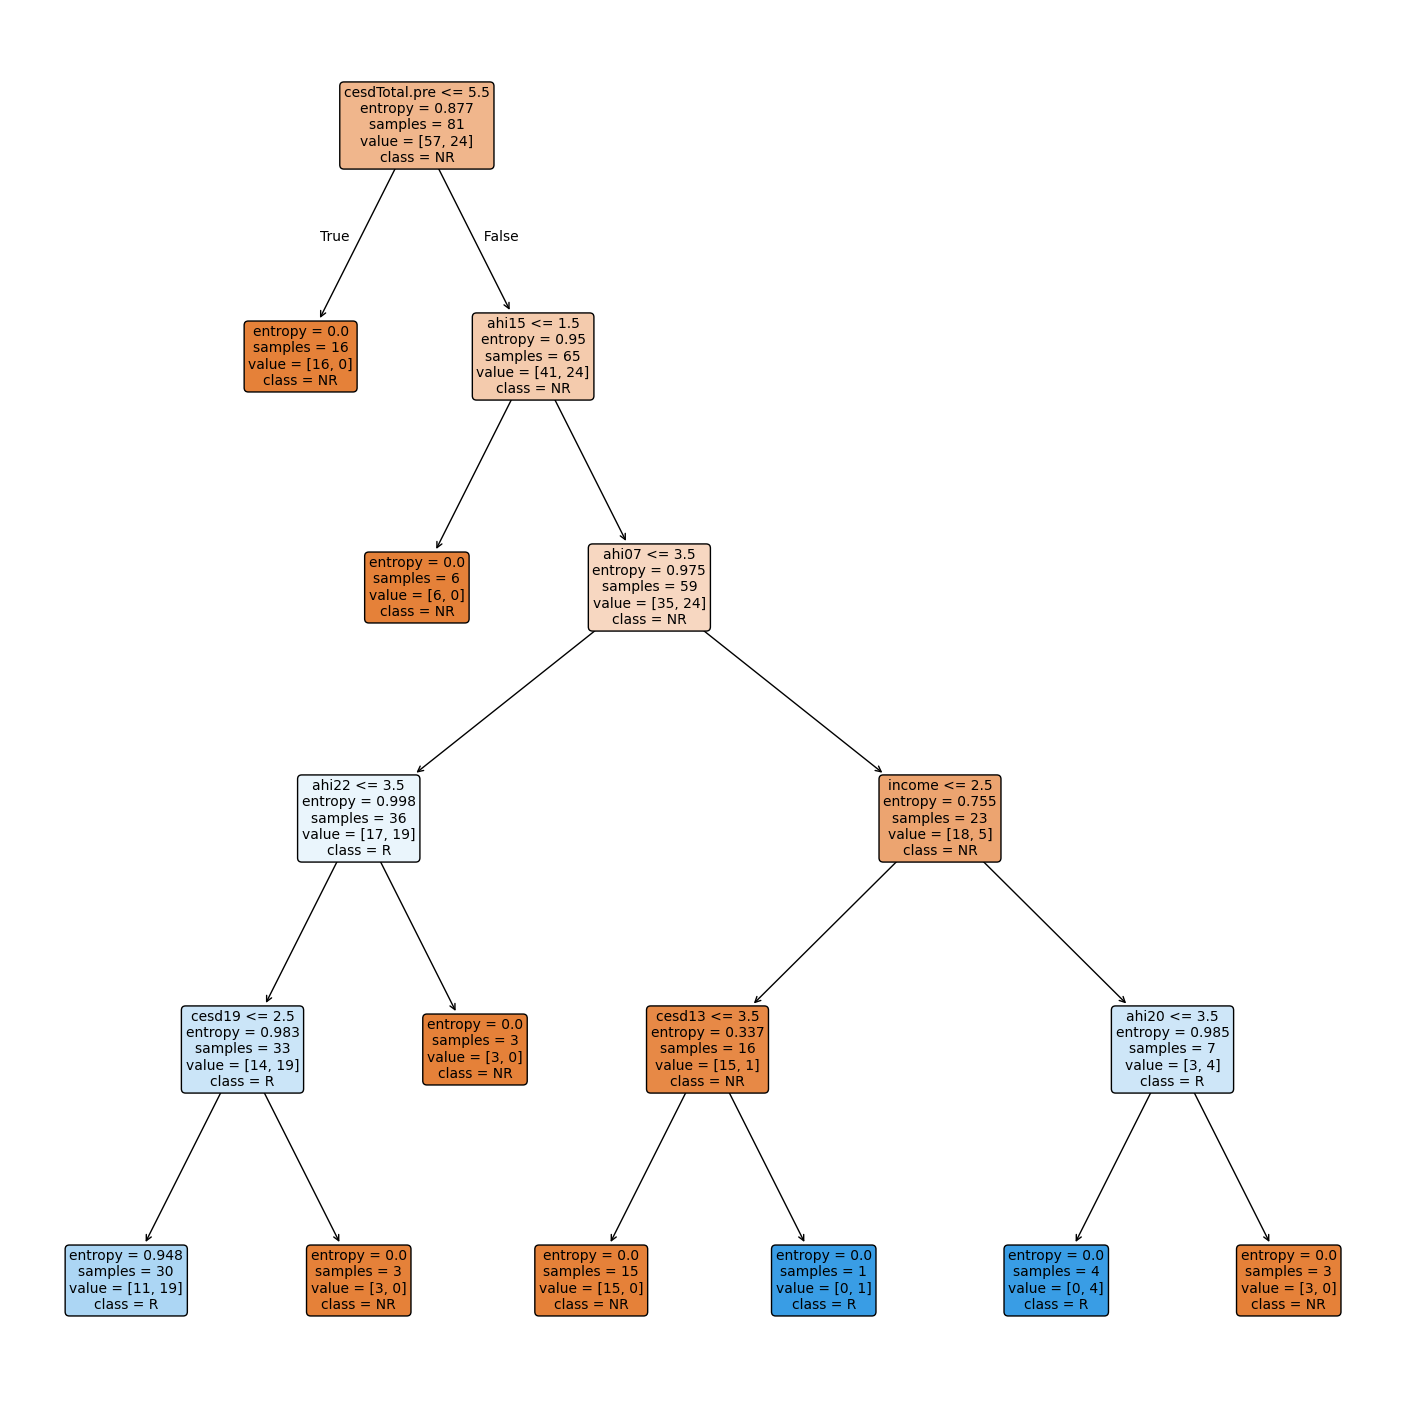
\includegraphics[width=\textwidth]{./03-exemplo/imagens/arvore.png}
    \caption{Modelo de árvore de decisão gerado.}
    \label{fig:arvore}
\end{figure}

A figura \ref{fig:matriz} apresenta a matriz de confusão com as classificações obtidas para o conjunto de dados de teste. O modelo construído foi capaz de predizer a melhora nos níveis de sintomas
depressivos das participantes do conjunto de dados de teste com uma acurária de $0,714$, precisão de $0,500$ e recall de $0,833$.

\begin{figure}[h]
    \centering
    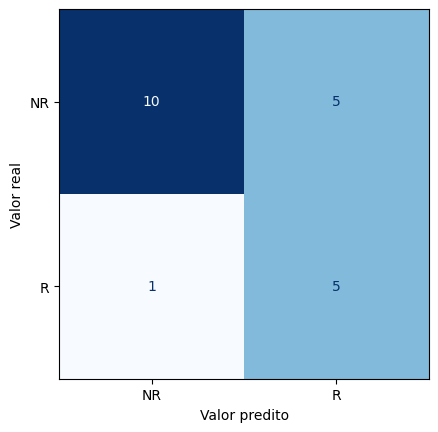
\includegraphics[width=0.5\textwidth]{./03-exemplo/imagens/matriz.png}
    \caption{Classificações para o conjunto de dados de teste.}
    \label{fig:matriz}
\end{figure}

Neste exemplo, buscou-se predizer melhora nos níveis de sintomas depressivos após uma intervenção de psicologia positiva via internet usando um modelo de aprendizagem de máquina do tipo árvore de
decisão. Foi possível, mesmo com um conjunto de dados de tamanho pequeno, construir um modelo funcional e com desempenho razoável, alcançando cerca de $70\%$ de acurácia. O resultado obtido alinha-se
com uma série achados recentes, onde, com técnicas similares, as características sociodemográficas e clínicas de pacientes foram usadas para predizer o desfecho de psicoterapia com sucesso \cite{Collins2023, Hornstein2021}.
A incorporação desse tipo de tecnologia na prática de psicoterapia permitiria a personalização de tratamentos com maiores níveis de assertividade: com auxílio de modelos de aprendizagem de máquina, o
psicoterapeuta poderia estimar as chances de sucesso de diversas intervenções a um custo relativamente baixo, escolhendo aquela que julgar mais adequada.

O modelo construído possui uma representação gráfica intuitiva que evidencia os critérios usados no processo de classificação das observações. A capacidade de inspecionar o funcionamento do modelo
é uma característica altamente desejável, pois permite que o psicoterapeuta use informações adicionais sobre o contexto do paciente para avaliar a qualidade da predição feitas pelo modelo, aumentando
a confiança nas decisões clínicas tomadas com auxílio desse tipo de tecnologia \cite{Stiglic2020, WHO2023}. A capacidade de interpretar as predições é uma característica particular de alguns tipos de modelos,
como as árvores de decisão; outras classes de modelos de aprendizagem de máquina não podem ser facilmente inspecionadas. As redes neurais artificiais, por exemplo, são uma classe de modelos de aprendizagem
de máquina que apresenta alta capacidade de aprendizagem e grande poder preditivo, mas não oferecem transparência em relação a seu funcionamento \cite{Stiglic2020}. A possibilidade de inspecionar classes
de modelos mais complexos é um problema de pesquisa em aberto e uma condição necessária para a implantação da tecnologia no contexto de atuação profissional em saúde mental \cite{Stiglic2020, WHO2023}.

Observa-se que o modelo final apresenta um viés de classificação que favorece a produção de falsos positivos, a atribuição da classe respondente a pacientes que não respondem ao tratamento. O viés fica evidente
na métrica de precisão de $50\%$: apenas metade das predições positivas produzidas pelo modelo estavam corretas. O surgimento do viés pode ser atribuído, em parte, ao pequeno número de observações disponíveis para
o treinamento do modelo. Além disso, grande parte das observações correspondiam a pacientes não respondentes, o que pode ter prejudicado a capacidade do modelo de identificar pacientes respondentes \cite{Delgadillo2020}.
Embora algumas técnicas de balanceamento de classes possam mitigar o problema \cite{Bi2019}, uma solução definitiva envolve necessariamente a obtenção de um conjunto de dados de treinamento maior e com distribuição
equilibrada entre as classes de desfecho \cite{Delgadillo2020}. O uso de modelos com esse tipo de viés poderia resultar em um grande número de pacientes encaminhados para intervenções com poucas chances de sucesso. O
encaminhamento falho tem consequências econômicas e clínicas negativas como o desperdício de recursos financeiros, o adiamento de um tratamento eficaz e a exposição a potenciais efeitos negativos do tratamento \cite{John2009}. 